\section{Modularisation}

\subsection{Multi-threading}

L'un des objectifs principaux est de pouvoir fonctionner sur plusieurs threads et donc d'exploiter au mieux les ressources des machines en notre possession. 
Notre objectif ici est de placer le moteur de jeu sur un thread, puis le moteur de rendu sur un autre
thread. Le moteur de rendu est nécessairement sur le thread principal (contraire matérielle), et le moteur
du jeu est sur un thread secondaire. Nous avons deux type d’information qui transite d’un module à l’autre :
les commandes et les notifications de rendu.

\subsection{La classe Client}

La classe Client contient les informations pour faire fonctionner le jeu : Mo-
teur de jeu (avec état intégré) et rendu.

\subsection{Serveur}

Pour jouer en réseau, nous allons mettre en place un serveur dont les classes sont présentées sur le schéma suivant. Ce dernier ne fonctionne pas mais nous avons commencé à coder les différentes classes de cette partie. 
Nous utilisons Json pour toutes les commandes qui vont transiter via le serveur. 

\begin{itemize}
    \item \textbf{Classe User et UserDB.}
    Ces deux classes permettent de simuler une petite base de données des joueurs qui seront en jeu sur le réseau. Dans un cas plus concret, ces classes feraient le lien avec une base de données SQL ou noSQL par exemple. Les méthodes comprises dans cette classe sont assez explicites et permettent des actions de base. 
    \newline 
    
    \item \textbf{Classe AbstractService}
    Cette classe abstraite gère la totalité du service REST du projet.
    
     \item \textbf{Classe Version Service et UserService}
     
     \item \textbf{Classe ServicesManager}. Il s'agit du gestionnaire de service, c'est à dire qu'il sélectionne le bon service et la bonne opération, exécute en fonction de l'URL et de la méthode HTTP. 
     
     \item \textbf{Classe ServicesException}
     Comme son nom l'indique, il gère les cas d'exceptions qui peuvent survenir afin de pouvoir interrompre l'exécution du service. 
     
     
\end{itemize} 

\begin{landscape}
    \begin{figure}[!htbp]
        \centering
        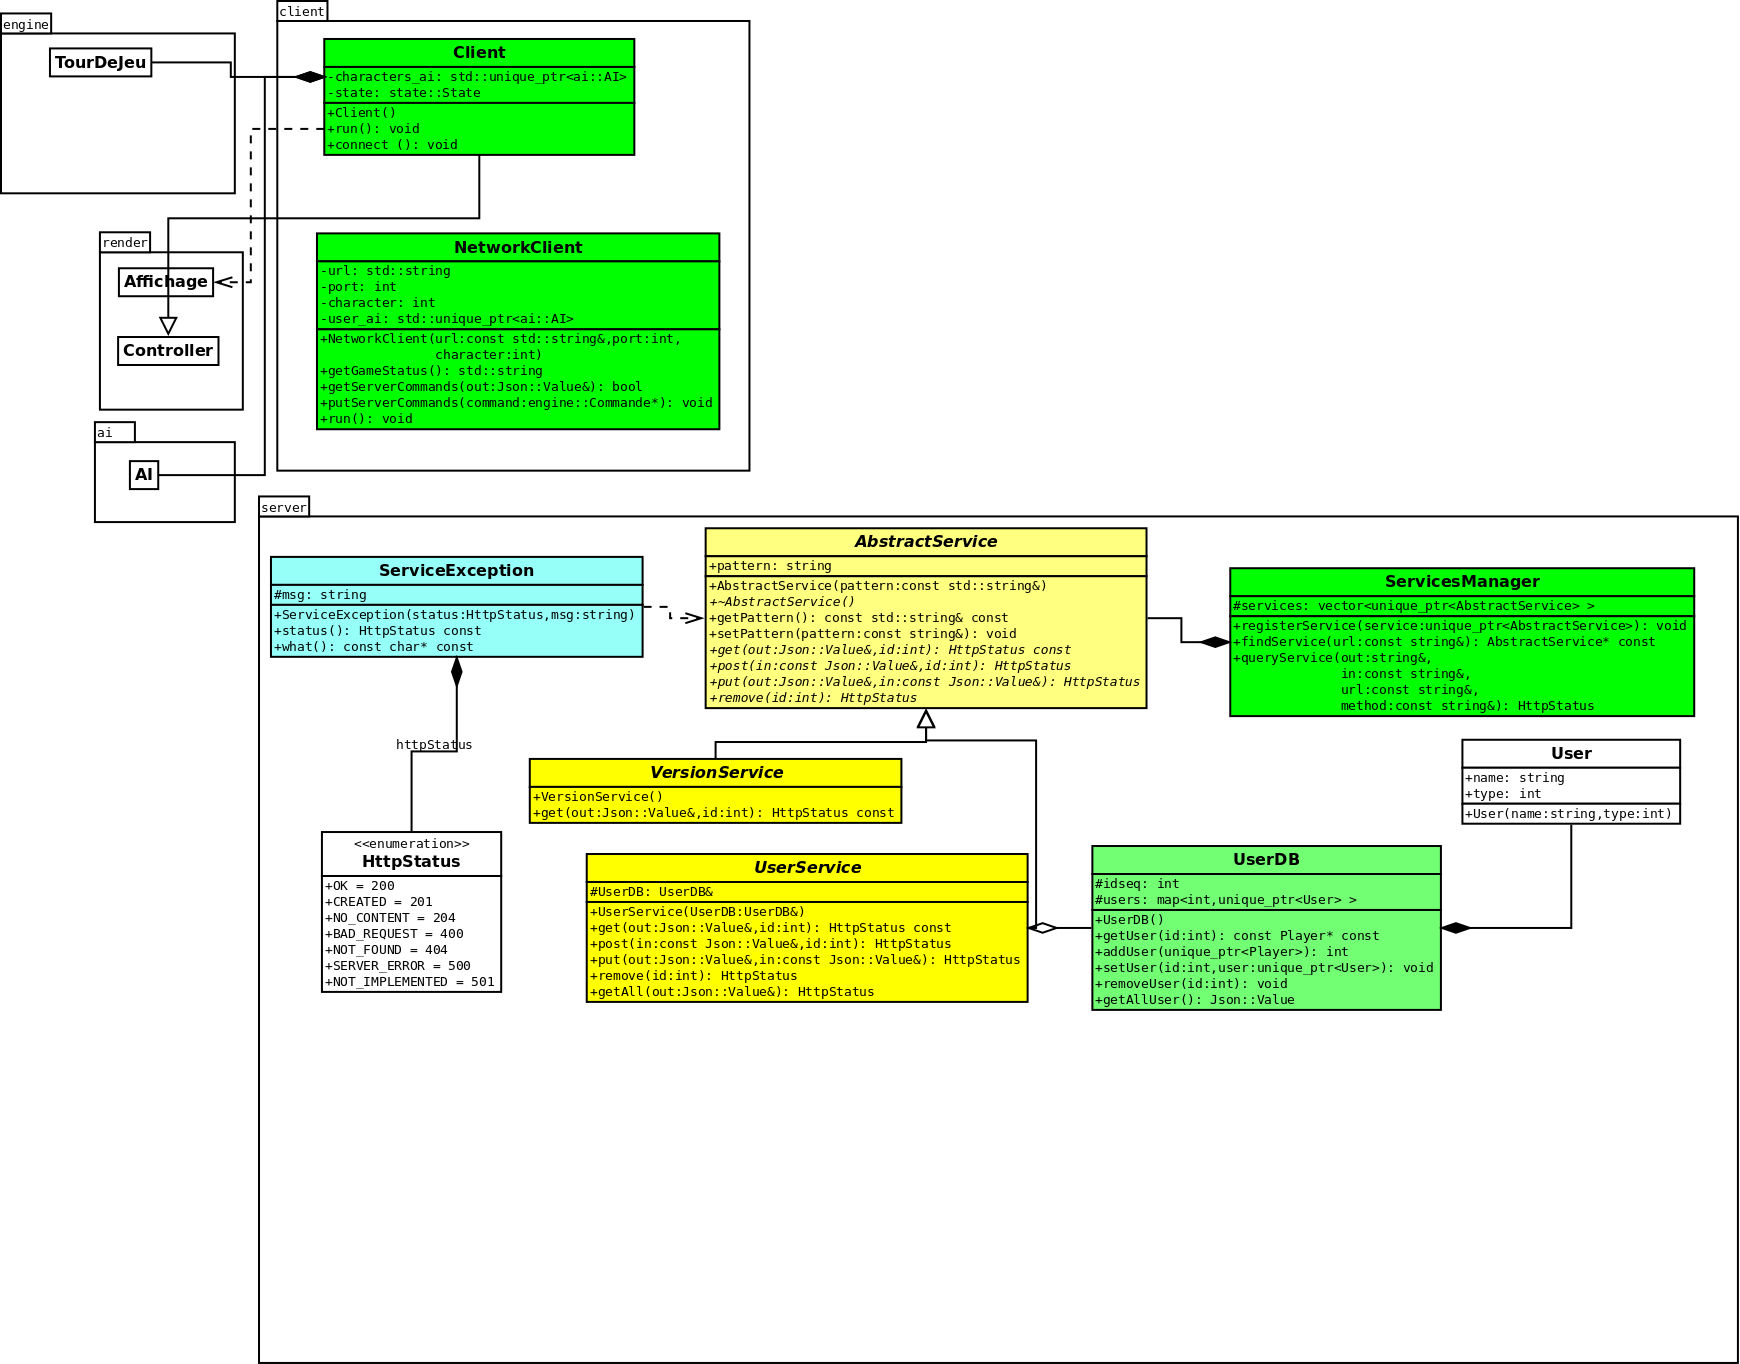
\includegraphics[width=17cm]{Images/module.png}
        \caption{Diagramme de la modularisation}
        \label{fig:ai}
    \end{figure}
\end{landscape}